% possible options include font size ('10pt', '11pt' and '12pt'),
%                          paper size ('a4paper', 'letterpaper', 'a5paper', 'legalpaper', 'executivepaper' and 'landscape') and
%                          font family ('sans' and 'roman')
\documentclass[11pt,a4paper,sans]{moderncv}
% adjust the page margins
\usepackage[scale=0.85]{geometry}
\usepackage{fontawesome}
% style options are 'casual' (default), 'classic', 'banking', 'oldstyle' and 'fancy'
\moderncvstyle{banking}
% color options 'black', 'blue' (default), 'burgundy', 'green', 'grey', 'orange', 'purple' and 'red'
\moderncvcolor{blue}
% to set the default font; use '\sfdefault' for the default sans serif font, '\rmdefault' for the default roman one, or any tex font name
\renewcommand{\familydefault}{\rmdefault}
% uncomment to suppress automatic page numbering for CVs longer than one page
\nopagenumbers{}
% if you want to change the width of the column with the dates
% \setlength{\hintscolumnwidth}{3cm}
% for the 'classic' style, if you want to force the width allocated to your name and avoid line breaks.
% be careful though, the length is normally calculated to avoid any overlap with your personal info; use this at your own typographical risks...
% \setlength{\makecvheadnamewidth}{10cm}
% Reduce name font size
% http://tex.stackexchange.com/questions/80428/name-in-a-single-line-in-moderncv
\renewcommand*{\namefont}{\fontsize{22}{29}\mdseries\upshape}

\usepackage{ifthen}
\usepackage{csquotes}
\MakeOuterQuote{"}

\definecolor{burgundy}{rgb}{0.596078,0,0} % taken from moderncv class
\definecolor{theblue}{rgb}{0.22,0.45,0.70} % taken from moderncv class
\usepackage{hyperref}
\hypersetup{
  bookmarks=false,
  unicode=false,          % non-Latin characters in Acrobat's bookmarks
  pdftoolbar=false,       % show Acrobat's toolbar?
  pdfmenubar=false,       % show Acrobat's menu?
  pdffitwindow=false,     % window fit to page when opened
  pdfstartview={FitH},    % fits the width of the page to the window
  pdftitle={Curriculum Vitae},              % title
  pdfauthor={Eduardo Mucelli Rezende Oliveira},     % author
  pdfsubject={Curriculum Vitae},   % subject of the document
  pdfcreator={LaTeX},     % creator of the document
  pdfproducer={Rubber},   % producer of the document
  pdfnewwindow=true,      % links in new window
  colorlinks=true,        % false: boxed links; true: colored links
  linkcolor=theblue,         % color of internal links
  citecolor=green,        % color of links to bibliography
  filecolor=magenta,      % color of file links
  urlcolor=theblue          % color of external links
}

\urlstyle{same}
% personal data
\name{Eduardo}{Mucelli}
\title{{\LARGE Software Engineer}}
\address{2 rue Niepce}{75014 Paris}{France}
\phone[mobile]{+33~787~361~492}
\email{edumucelli@gmail.com}
\social[linkedin]{edumucelli}
\social[github]{edumucelli}
\extrainfo{\small{\faCode}~\href{https://code.launchpad.net/~eduardo-mucelli}{eduardo-mucelli}}
% \photo[64pt][0.4pt]{oui}                       % optional, remove / comment the line if not wanted; '64pt' is the height the picture must be resized to, 0.4pt is the thickness of the frame around it (put it to 0pt for no frame) and 'picture' is the name of the picture file

% bibliography adjustements (only useful if you make citations in your resume, or print a list of publications using BibTeX)
%   to show numerical labels in the bibliography (default is to show no labels)
% \makeatletter\renewcommand*{\bibliographyitemlabel}{\@biblabel{\arabic{enumiv}}}\makeatother
%   to redefine the bibliography heading string ("Publications")
%\renewcommand{\refname}{Articles}

% bibliography with mutiple entries
%\usepackage{multibib}
%\newcites{book,misc}{{Books},{Others}}
% ==================
% Boolean flags

\newboolean{en}
\setboolean{en}{true}           % true gera curriculo em ingles
\newboolean{pt}
\setboolean{pt}{false}          % true gera curriculo em portugues

\newboolean{academy}            % this curriculum focus a company, or academy?
\setboolean{academy}{true}

\newboolean{everything}
\setboolean{everything}{false}  % false gera curriculo so com as coisas mais recentes

% ==================

\newcommand{\course}{\ifthenelse{\boolean{en}}      {Course}{Curso}}
\newcommand{\type}{\ifthenelse{\boolean{en}}        {Type}{Tipo}}
\newcommand{\period}{\ifthenelse{\boolean{en}}      {Period}{Período}}
\newcommand{\institution}{\ifthenelse{\boolean{en}} {Institution}{Instituição}}
\newcommand{\avgscore}{\ifthenelse{\boolean{en}}    {Avg.Score}{Nota Média}}
\newcommand{\score}{\ifthenelse{\boolean{en}}       {Score}{Nota}}
\newcommand{\area}{\ifthenelse{\boolean{en}}        {Area}{Área}}
\newcommand{\project}{\ifthenelse{\boolean{en}}     {Project}{Projeto}}
\newcommand{\pdescription}{\ifthenelse{\boolean{en}}{Description}{Descrição}}

\newcommand{\ufmg}{\ifthenelse{\boolean{en}}        {Federal University of Minas Gerais}{Universidade Federal de Minas Gerais}}
\newcommand{\puc}{\ifthenelse{\boolean{en}}         {Pontifical Catholic University of Minas Gerais}{Pontifícia Universidade Católica de Minas Gerais}}
\newcommand{\ecole}{\ifthenelse{\boolean{en}}       {École Polytechnique}{École Polytechnique}}

\newcommand{\ufmglinked}{\ifthenelse{\boolean{en}}  {\href{http://www.ufmg.br}{Federal University of Minas Gerais}}
                                                                              {Universidade Federal de Minas Gerais}}
\newcommand{\puclinked}{\ifthenelse{\boolean{en}}   {\href{http://www.pucminas.br}{Pontifical Catholic University of Minas Gerais}}
                                                                                  {Pontifícia Universidade Católica de Minas Gerais}}
\newcommand{\ecolelinked}{\ifthenelse{\boolean{en}} {\href{http://www.polytechnique.edu}{École Polytechnique}}
                                                    {\href{http://www.polytechnique.edu}{École Polytechnique}}}

\newcommand{\france}{\ifthenelse{\boolean{en}}      {France}{França}}
\newcommand{\brazil}{\ifthenelse{\boolean{en}}      {Brazil}{Brasil}}

\newcommand{\january}{\ifthenelse{\boolean{en}}     {January }{Janeiro }}
\newcommand{\february}{\ifthenelse{\boolean{en}}    {February }{Fevereiro }}
\newcommand{\march}{\ifthenelse{\boolean{en}}       {March }{Março }}
\newcommand{\april}{\ifthenelse{\boolean{en}}       {April }{Abril }}
\newcommand{\may}{\ifthenelse{\boolean{en}}         {May }{Maio }}
\newcommand{\june}{\ifthenelse{\boolean{en}}        {June }{Junho }}
\newcommand{\july}{\ifthenelse{\boolean{en}}        {July }{Julho }}
\newcommand{\august}{\ifthenelse{\boolean{en}}      {August }{Agosto }}
\newcommand{\september}{\ifthenelse{\boolean{en}}   {September }{Setembro }}
\newcommand{\october}{\ifthenelse{\boolean{en}}     {October }{Outubro }}
\newcommand{\november}{\ifthenelse{\boolean{en}}    {November }{Novembro }}
\newcommand{\december}{\ifthenelse{\boolean{en}}    {December }{Dezembro }}
\newcommand{\cc}{\ifthenelse{\boolean{en}}          {Computer Science}{Ciência da Computação}}
\newcommand{\bachelor}{\ifthenelse{\boolean{en}}    {Bachelor's degree}{Bacharelado}}
\newcommand{\master}{\ifthenelse{\boolean{en}}      {Master's degree}{Mestrado}}
\newcommand{\phd}{\ifthenelse{\boolean{en}}         {Ph.D}{Doutorado}}
\newcommand{\wsn}{\ifthenelse{\boolean{en}}         {Wireless Sensor Networks}{Redes de Sensores sem Fio}}
\newcommand{\complex}{\ifthenelse{\boolean{en}}     {Complex Networks}{Redes Complexas}}
\newcommand{\data}{\ifthenelse{\boolean{en}}        {Large-scale Data Analysis}{Análisa de Dados em Larga Escala}}
\newcommand{\research}{\ifthenelse{\boolean{en}}    {Research}{Pesquisa}}
\newcommand{\pand}{\ifthenelse{\boolean{en}}        {and }{e }}

\newcommand{\awards}{\ifthenelse{\boolean{en}}      {Awards}{Prêmios}}

\newcommand{\jobtitle}{\ifthenelse{\boolean{en}}    {Job Title}{Cargo}}
\newcommand{\company}{\ifthenelse{\boolean{en}}     {Company}{Empresa}}
\newcommand{\se}{\ifthenelse{\boolean{en}}          {Software Engineer}{Engenheiro de Software}}
\newcommand{\mg}{\ifthenelse {\boolean{en}}         {Minas Gerais, Brazil}{Minas Gerais, Brasil}}
\newcommand{\paris}{\ifthenelse {\boolean{en}}      {Paris, France}{Paris, França}}
\newcommand{\venice}{\ifthenelse {\boolean{en}}     {Venice, Italy}{Veneza, Itália}}

\newcommand{\english}{\ifthenelse{\boolean{en}}     {English}{Inglês}}
\newcommand{\portuguese}{\ifthenelse{\boolean{en}}  {Portuguese}{Português}}
\newcommand{\italian}{\ifthenelse{\boolean{en}}     {Italian}{Italiano}}
\newcommand{\french}{\ifthenelse{\boolean{en}}      {French}{Francês}}

\newcommand{\languages}{\ifthenelse{\boolean{en}}   {Language}{Linguagen}}
\newcommand{\planguage}{\ifthenelse{\boolean{en}}   {Language}{Linguagem}}
\newcommand{\vcs}{\ifthenelse{\boolean{en}}         {VCS}{SCV}}
\newcommand{\db}{\ifthenelse{\boolean{en}}          {DB}{BD}}
\newcommand{\methodologies}{\ifthenelse{\boolean{en}}{Methodo\-logies}{Metodo\-logias}}
\newcommand{\os}{\ifthenelse{\boolean{en}}          {OS}{SO}}
\newcommand{\other}{\ifthenelse{\boolean{en}}       {Others}{Outras}}
\newcommand{\crawling}{\ifthenelse{\boolean{en}}    {Web crawlers}{Web crawlers}}
\newcommand{\inter}{\ifthenelse{\boolean{en}}       {Internationalization }{Internationalização }}
\newcommand{\pattern}{\ifthenelse{\boolean{en}}     {Design Patterns}{Padrões de Projeto}}

\newcommand{\ptitle}{\ifthenelse{\boolean{en}}      {Title}{Título}}
\newcommand{\issuer}{\ifthenelse{\boolean{en}}      {Issuer}{Emissor}}

% ==================

\begin{document}

\begin{minipage}[t]{.84\linewidth}
  \makecvtitle
  \vspace{-1cm}
\end{minipage}
\begin{minipage}[c]{.16\linewidth} % set percentage of line width as desired
  \fcolorbox{theblue}{white}{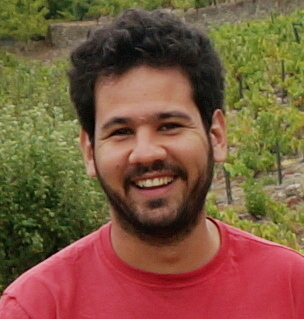
\includegraphics[width=70pt]{photo_1_a.JPG}} %set scale as desired, picture named profile.png
\end{minipage}
\ifthenelse {\boolean{en}} {
 	\ifthenelse {\boolean{everything}} {
 		\section{Education}
 		} {
 		\section{Recent Education}
 		}
    } {
		\ifthenelse {\boolean{everything}} {
	 		\section{Educa��o}
	 	} {
	 		\section{Educa��o recente}
	 	}
    }
	\begin{tabularx}{0.97\linewidth}{>{\raggedleft\scshape}p{2.1cm}X}
		\gray \course & \textbf{\cc} \\
		\gray \type & \textbf{\phd} \\
		\gray \period & \textbf{\october 2011 --- \may 2015} \\
		\gray \institution & \textbf{\ecolelinked} {\hfill \france} \\
		& % quebra de linha na gambiarra
	\end{tabularx}

	\begin{tabularx}{0.97\linewidth}{>{\raggedleft\scshape}p{2.1cm}X}
		\gray \course & \textbf{\cc} \\
		\gray \type & \textbf{\master} \\
		\gray \period & \textbf{\march 2009 --- \july 2011} \\
		\gray \institution & \textbf{\ufmglinked} {\hfill \brazil} \\
	    \gray \avgscore & \textbf{94}\% \\
		& % quebra de linha na gambiarra
	\end{tabularx}

	\begin{tabularx}{0.97\linewidth}{>{\raggedleft\scshape}p{2.1cm}X}
		\gray \course & \textbf{\cc} \\
		\gray \type & \textbf{\bachelor} \\
		\gray \period	& \textbf{\august 2004 --- \august 2008} \\
		\gray \institution & \textbf{\puclinked} {\hfill \brazil} \\
	    \gray \avgscore & \textbf{85}\% \\
		& % quebra de linha na gambiarra
	\end{tabularx}

\section{Skills}

\cvdoubleitem{\protect\languages}{Python, Ruby, R, Javascript, Java \pand Swift}{\protect\db}{MySQL, PostgreSQL (PostGIS), \pand Cassandra}
\cvdoubleitem{\protect\vcs}{Subversion, Git, \pand Bazaar}{\protect\os}{Linux, Android \pand OS X}
\cvdoubleitem{Framework}{Ruby on Rails, jQuery, Zurb Foundation, \pand Semantic-UI}{\protect\other}{Machine learning, full-stack development, REST API development, \pand \crawling } % D-Bus
\ifthenelse{\boolean{en}}{\section{Languages}}{\section{Idiomas}}

\cvdoubleitem{\protect\portuguese}{Native speaker}{\protect\french}{Advanced}
\cvdoubleitem{\protect\english}{Fluent}{\protect\italian}{Advanced}
\section{Professional Experiences}
\newcommand*{\cvsimple}[4][.25em]{
\begin{tabular*}{\maincolumnwidth}{l@{\extracolsep{\fill}}r}%
	% {\bfseries #4} & {\bfseries #5}\\%
	{\itshape #3} & {\itshape #2}\\%
\end{tabular*}%
\ifx&#4&%
\else{\\%
	\begin{minipage}{\maincolumnwidth}%
		\small#4%
\end{minipage}}\fi%
\par\addvspace{#1}}

\cventry{\january 2023 -- Present}{\sse}{Synthesia}{Remote}{}{
	Working on improving the robustness of the video generation.
}
\cventry{\december 2021 -- \november 2022}{\seii}{Canonical}{Remote}{}{
	Improving the data pipeline Python codebase to serve technical and non-technical internal teams.
	Working on the service behind \href{https://ubuntu.com/security/livepatch}{Livepatch} in Golang.
}
% Add second entry to the same company https://tex.stackexchange.com/a/294612
\cvsimple{\june 2020 -- \november 2021}{\se}{
	Working on the services behind \href{https://ubuntu.com/advantage}{Ubuntu Advantage} in Golang and Python.
	Introduced a BDD suite to our main Golang services.
	Revamping team's data pipelines: large refactoring of the Python codebase, type checking, linting, moving from Openstack to Kubernetes (Argo), Grafana, Prometheus, Pushgateway, alerting.
}
\cventry{\july 2016 -- \may 2020}{\se}{BlaBlaCar}{\protect\france}{}{
	Developed features, optimized performance, deployed and monitored a dozen of Java services at the Trip Search team. \href{https://medium.com/blablacar-tech/fast-machine-learning-predictions-6856b3623e5}{Wrote and integrated the first library} to handle Machine Learning predictions at scale for \href{https://github.com/edumucelli/benchmark-xgboost-java}{which I have extensively measured performance}. Significantly worked on the \href{https://blog.blablacar.com/newsroom/news-list/new-search-logo-visual-identity}{new search, routing and matching algorithm}. Main technologies were Java, Elasticsearch, PostgreSQL, PostGIS, XGBoost, OSRM, MySQL and Redis, R and Python.
}
\cventry{\june 2015 -- \june 2016}{Postdoctoral Researcher}{Orange}{\protect\france}{}{
	Developed machine-learning assisted techniques to predict users' QoE based on network's KPIs.
}
\cventry{\july 2011 --- \september 2011}{\se}{Dito Internet}{\protect\brazil}{}{
	Developed in Ruby on Rails, as part of a team, Telecom Italia Mobile's project called TIM Beta, \textit{\href{www.timbeta.com.br}{timbeta.com.br}}.
}
\cventry{\november 2010 --- \may 2011}{Researcher Intern}{Telecom Italia Future Centre}{\protect\italy}{}{
	Developed, in Python, a project called Future of Enterprises aiming to improve the real-time interaction among employees.
}
\cventry{\february 2008 --- \february 2009}{\se}{Task Internet}{\protect\brazil}{}{
	Lead developer of a social network in Ruby on Rails.
}
\ifthenelse {\boolean{en}}
  {\section{Web Applications} \label{sec:web_app}}
  {\section{Aplicativos Web} \label{sec:web_app}}

\cvitem{}{\textbf{Easy Bike} -- \url{http://easy.bike}} \label{easy_bike}
\cvitem{}{Ruby, Python, \pand Javascript}
% \cvitem{URL}{\url{http://easy.bike}}
\cvitem{}{It finds the best cycling routes using bike-sharing systems in more than 390 cities distributed in 42 countries. It considers real-time information of how many bicycles are available closest to you and how many available bike stands are available in the stations close to the destination address. It then chooses the best stations and route for you. Besides, it provides city-specific domains such as \href{http://paris.easy.bike}{paris.easy.bike}, \href{http://london.easy.bike}{london.easy.bike}, or \href{http://ny.easy.bike}{ny.easy.bike}, etc., to directly access the service in the respective cities.}

\cvitem{}{\textbf{Proconfie} -- \url{http://www.proconfie.com}} \label{proconfie}
\cvitem{}{Ruby, Python, \pand R}
\cvitem{}{It helps people to choose companies based on historical problems presented with other customers. Received Honorary Mention award from the Brazilian Ministry of Justice. Refer to Section \hyperref[sec:awards]{Awards} for further information.}

\cvitem{}{\textbf{CEP Aberto} -- \url{http://www.cepaberto.com}}
\cvitem{}{Ruby, Python, \pand Javascript}
\cvitem{}{Collaborative application that aims to publicly open the Brazilian Postal Code (CEP) data. It currently contains information of about 1 million CEPs. It provides an API for developers willing to use geolocalized Postal Code data and, for the end-users, the possibility to edit, add, fix, follow, etc, specific postal-coded-locations in order to improve the quality of the data. About a thousand of registered users.}
\ifthenelse {\boolean{en}}
  {\section{Some Open Source Projects} \label{sec:open_source}}
  {\section{Alguns Projetos \textit{Open Source}} \label{sec:open_source}}

\cvitem{}{\textbf{Twitter applet} -- Code \href{https://code.launchpad.net/\~eduardo-mucelli/cairo-dock-plug-ins-extras/Twitter}{\scriptsize\faLink}}
% \cvitem{}{\textbf{\ifthenelse {\boolean{en}}{Python using OAuth}{Python usando OAuth}}}
\cvitem{}{\ifthenelse {\boolean{en}}
	                      {Twitter applet for Cairo-Dock with real-time personal tweet alert and many of the capabilities provided by Twitter's API.}
	                      {Mini-aplicativo Twitter para o Cairo-Dock com alerta de tweets pessoais em tempo real e muitas outras funcionalidades providas pela API do Twitter.}}

\cvitem{}{\textbf{WebSearch applet} -- Code \href{https://code.launchpad.net/\~eduardo-mucelli/cairo-dock-plug-ins-extras/WebSearch}{\scriptsize\faLink}}
% \cvitem{}{\textbf{Ruby}}
\cvitem{}{\ifthenelse {\boolean{en}}
      					{Metasearch applet for Cairo-Dock capable of retrieving text and image results from several sources, e.g., Google, Bing, Yahoo!, Youtube, and Twitter.}
	        			{Mini-aplicativo de Meta-Busca para o Cairo-Dock com a capacidade de buscar resultados de diversas fontes, e.g., Google, Bing, Yahoo!, Youtube e Twitter.}}

\cvitem{}{\textbf{Repeat One Song} -- Code \href{https://launchpad.net/repeat-one-song}{\scriptsize\faLink}}
% \cvitem{}{\textbf{Python}}
\cvitem{}{\ifthenelse {\boolean{en}}
      					{The Repeat One Song feature for Rhythmbox.}
                      	{A funcionalidade de repetir uma música para o Rhythmbox.}}

% \begin{tabularx}{0.97\linewidth}{>{\raggedleft\scshape}p{2.1cm}X}
% 	\gray \ptitle & \textbf {RubyBikes} \\
%     \gray \planguage & \textbf {Ruby} (Code \href{https://github.com/eduardom}{code}) \\
% 		%\gray URL & \textbf{\url{https://launchpad.net/rhythmidgin}} \\
% 			& \ifthenelse {\boolean{en}}
%                       {Ruby Gem that scrapes and aggregates real-time information of bike-sharing systems around the world.}
%                       {Gem Ruby que coleta e agrega informação em tempo real de sistemas de bicicletas públicas do mundo todo.} \\
%             &
% \end{tabularx}

\cvitem{}{\textbf{Translator} -- Code \href{https://code.launchpad.net/\~eduardo-mucelli/cairo-dock-plug-ins-extras/Translator}{\scriptsize\faLink}}
% \cvitem{}{\textbf {\ifthenelse {\boolean{en}}{Python using SGMLParser}{Python usando SGMLParser}}}
\cvitem{}{\ifthenelse {\boolean{en}}
      					{Full-featured Google Translator-based translator applet for Cairo-Dock.}
						{Mini-aplicativo tradutor para o Cairo-Dock baseado no Google Translator.}}


\cvitem{}{\textbf{Quote} -- Code \href{https://code.launchpad.net/\~eduardo-mucelli/cairo-dock-plug-ins-extras/Quote}{\scriptsize\faLink}}
% \cvitem{}{\textbf {\ifthenelse {\boolean{en}}{Python using SGMLParser}{Python usando SGMLParser}}}
\cvitem{}{\ifthenelse {\boolean{en}}
      					{"Quote of the day" applet for Cairo-Dock. It crawls Internet sources, e.g., Bash.org, Xkcdb.com, Qdb.us, and more.}
                      	{Mini-aplicativo Frase do Dia para o Cairo-Dock. Busca frases de vários sites como, por exemplo, Bash.org, Xkcdb.com, Qdb.us, e mais.}}

\ifthenelse {\boolean{everything}} {
	\cvitem{}{\textbf{Rhythmidgin} -- Code \href{https://launchpad.net/rhythmidgin}{\scriptsize\faLink}}
	% \cvitem{}{\textbf{Python}}
	\cvitem{}{\ifthenelse {\boolean{en}}
      						{Show to Pidgin buddies what is the song you're listening to with Rhythmbox.}
							{Mostra para os contatos do Pidgin qual a música que você está escutando pelo Rhythmbox.}}

	\cvitem{}{\textbf{Liferea} -- Code \href{https://code.launchpad.net/\~eduardo-mucelli/cairo-dock-plug-ins-extras/Liferea}{\scriptsize\faLink}}
	% \cvitem{}{\textbf{Python}}
	\cvitem{}{\ifthenelse {\boolean{en}}
      						{Applet that provides to Cairo-Dock an interface with Liferea feed news aggregator.}
                      		{Mini-aplicativo que fornece ao Cairo-Dock uma interface ao agreagador de feed Liferea.}}
}{}
\ifthenelse {\boolean{en}} {
	\ifthenelse {\boolean{everything}} {
		\section{\href{https://scholar.google.com/citations?user=pD4KMUsAAAAJ}{Publications~\scriptsize\faLink}}
	}{
		\section{Recent \href{https://scholar.google.com/citations?user=pD4KMUsAAAAJ}{publications~\scriptsize\faLink}}
	}
} {
	\ifthenelse {\boolean{everything}} {
		\section{\href{https://scholar.google.com/citations?user=pD4KMUsAAAAJ}{Publicações~\scriptsize\faLink}}
	} {
		\section{\href{https://scholar.google.com/citations?user=pD4KMUsAAAAJ}{Publicações~\scriptsize\faLink} recentes}
	}
}
\begin{itemize}
% \item \cvitem{}{Lin, Yu-Ting and Oliveira, Eduardo Mucelli Rezende and Ben Jemaa, Sana and Eddine Elayoubi, Salah., \emph{"Machine Learning for Predicting QoE of Video Streaming in Mobile Networks"}, IEEE ICC Communication QoS, reliability and modeling symposium, May 2017.}
\item \cvitem{}{Oliveira, Eduardo Mucelli Rezende and Carneiro Viana, Aline and Naveen, K. P. and Sarraute, Carlos., \emph{"Mobile Data Traffic Modeling: Revealing Temporal Facets"}, Elsevier Computer Networks, November 2016.}
\item \cvitem{}{Oliveira, Eduardo Mucelli Rezende and Carneiro Viana, Aline and Naveen, K. P. and Sarraute, Carlos and Brea, Jorge and Alvarez-Hamelin, Ignacio., \emph{"On the regularity of human mobility"}, Elsevier Pervasive and Mobile Computing, May 2016.}
\ifthenelse {\boolean{long}} {
	\item \cvitem{}{Oliveira, Eduardo Mucelli Rezende and Carneiro Viana, Aline and Naveen, K. P. and Sarraute, Carlos., \emph{"Analysis and Modeling of Mobile Data Traffic in Mexico City"}, NetMob, April 2015, Mit Media Lab, Cambridge, MA, United States.}
	\item \cvitem{}{Oliveira, Eduardo Mucelli Rezende and Carneiro Viana, Aline and Naveen, K. P. and Sarraute, Carlos., \emph{"Measurement-driven mobile data traffic modeling in a large metropolitan area"}, IEEE Percom, March 2015, Saint Louis, United States.}
	\item \cvitem{}{Oliveira, Eduardo Mucelli Rezende and Viana, Aline Carneiro., \emph{"From Routine to Network Deployment for Data Offloading in Metropolitan Areas"}, IEEE SECON, June 2014, Singapore.}
	\item \cvitem{}{Oliveira, Eduardo Mucelli Rezende and Viana, Aline Carneiro., \emph{"Routine-based Network Deployment"}, IEEE INFOCOM, Student workshop, April 2014, Toronto, Canada.}
	\item \cvitem{}{Oliveira, Eduardo Mucelli Rezende and Viana, Aline Carneiro., \emph{"From Routine To Better Network Services"}, IEEE/IFIP WMNC, May 2014, Algarve, Portugal.}
	\item \cvitem{}{Oliveira, Eduardo Mucelli Rezende and Viana, Aline Carneiro., \emph{"Routine-based network deployment for data offloading in metropolitan areas"}, IEEE WCNC 2014, Istanbul, Turkey.}
	\ifthenelse {\boolean{everything}} {
		\item \cvitem{}{Oliveira, Eduardo Mucelli Rezende and Viana, Aline Carneiro., \emph{"From your routine to hotspot deployment for data offloading"}, ACM CoNEXT Student 2012, Nice, France.}
		\item \cvitem{}{Oliveira, Eduardo M. R., Ramos, Heitor S., Loureiro, Antonio A. F., \emph{"Centrality-based routing for Wireless Sensor Networks"}, IEEE Wireless Days (WD), 2010 IFIP, Venice, Italy.}
		\item \cvitem{}{Oliveira, Eduardo Mucelli Rezende, O. S. V. M., Pedro, Mini, R. A. F. Comunicação, Codificação e Fusão de Dados para uma Aplicação de Detecção de Incêndios utilizando Redes de Sensores sem Fio \emph{"Data Codification, Fusion and Communication in Wireless Sensors Networks"}, 1º Workshop on Pervasive and Ubiquitous Computing, 2007, Gramado, RS, Brazil.}
	}{}
}{}
\end{itemize}
\ifthenelse{\boolean{en}} {\section{Awards}\label{sec:awards}}
                          {\section{Prêmios}\label{sec:awards}}
	
	\begin{tabularx}{0.97\linewidth}{>{\raggedleft\scshape}p{2.1cm}X}
		\gray \ptitle & \textbf{\ifthenelse{\boolean{en}}{Honorary mention}{Menção honrosa}} \\
		\gray \issuer & \textbf{\ifthenelse{\boolean{en}}{Brazilian Ministry of Justice}{Ministério da Justiça}} \\
		\gray \ifthenelse{\boolean{en}}{Date}{Data} & \textbf{\may 2013} \\
		      & \ifthenelse{\boolean{en}}
		        {Open Data Applications Contest. Lead developer of a Ruby on Rails application called Proconfie. Refer to the Section \hyperref[sec:web_app]{Web Applications} for more details about \hyperref[proconfie]{Proconfie}.}
		        {1\textsuperscript{o} Concurso de Aplicativos do Ministério da Justiça. Desenvolvedor do aplicativo Proconfie. Veja a seção \hyperref[sec:web_app]{Aplicativos Web} para mais detalhes sobre o \hyperref[proconfie]{Proconfie}.} \\
		&
	\end{tabularx}
	
	\begin{tabularx}{0.97\linewidth}{>{\raggedleft\scshape}p{2.1cm}X}
		\gray \ptitle & \textbf{\ifthenelse{\boolean{en}}{Silver Medal}{Medalha de Prata}} \\
		\gray \issuer & \textbf{\puc} \\
		\gray \ifthenelse{\boolean{en}}{Date}{Data} & \textbf{\july 2008} \\
		      & \ifthenelse{\boolean{en}}
		        {Second best overall score during the bachelor.}
		        {Segunda melhor nota total durante todo a graduação.} \\
		&
	\end{tabularx}
	
	\begin{tabularx}{0.97\linewidth}{>{\raggedleft\scshape}p{2.1cm}X}
		\gray \ptitle & \textbf{\ifthenelse{\boolean{en}}{Honorary mention}{Menção honrosa}} \\
		\gray \issuer & \textbf{\puc} \\
		\gray \ifthenelse{\boolean{en}}{Date}{Data} & \textbf{\may 2007} \\
		      & \ifthenelse{\boolean{en}}
		        {For the work "Game Theory in Decision Making in Wireless Sensor Networks" presented in the 15\textsuperscript{th} Sciences Seminar.}
				{Para o trabalho "Teoria dos Jogos na Tomada de Decisão em Redes de Sensores Sem Fio" apresentado no 15\textsuperscript{o} Seminário de Ciências Exatas.} \\
		&
	\end{tabularx}

\section{Hobbies}
\cvitem{Music}{Amateur drummer for 2 years and currently playing pandeiro (Brazilian percussion).}
\cvitem{Sport}{Swimming, BMX, soccer player on a youth professional team for 5 years, Brazilian dancing lessons for 3 years.}
\cvitem{Photography}{Specially Moon, and macro of flowers.}
% \clearpage
% %-----       letter       ---------------------------------------------------------
% recipient data
% \recipient{Company Recruitment team}{Company, Inc.\\123 somestreet\\some city}
\recipient{Dailymotion team}{}
\date{\today}
\opening{Dear Sir or Madam,}
\closing{Yours faithfully,}
% \enclosure[Attached]{curriculum vit\ae{}}          % use an optional argument to use a string other than "Enclosure", or redefine \enclname
\makelettertitle

I am a Ph.D. in Computer Science at École Polytechnique, France. My Thesis tackled characterization, planning, and deployment problems of urban wireless networks using large-scale datasets of human mobility and data traffic. Besides, I am Linux and Open Source enthusiast for 15 years now. I have \hyperref[sec:open_source]{several projects}, created on my spare time.

Furthermore, I have made the full-stack development of \hyperref[sec:web_app]{three web applications}. E.g., from the \textit{"\href{http://easy.bike}{Easy.Bike}'s"} real-time back-end crawlers, R-based statistics on \textit{"\href{http://www.proconfie.com}{Proconfie}"}, to the front-end on \textit{"\href{http://www.cepaberto.com}{CEP Aberto}"}, and the Apache and MySQL fine-tuning for the three of them within the same VPS.

% Briefly, the first, \textit{"\href{http://easy.bike}{Easy.Bike}"} is a free application that helps bike-sharing cyclers to find the best bicycle stations and route from their places to their destinations. The second, \textit{"\href{http://www.proconfie.com}{Proconfie}"}, is a free application that helps people to choose companies based on historical problems presented with other customers. It received Honorary Mention award from the Brazilian Ministry of Justice. Finally, \textit{"\href{http://www.cepaberto.com}{CEP Aberto}" (Open Postal Code)} is a free and collaborative application that aims to open publicly the Postal Code geolocalized data in Brazil, which even after several popular requests, can be only accessed by those who pay an absurd amount of money for the Brazilian Post-mail service. It provides an API for developers willing to use the Postal Code data and, for the end-users, the possibility to edit, add, fix, follow, specific postal-coded-locations in order to improve the quality of the data.

% I have worked and experienced multicultural environments. I was born in Brazil, coursed part of my Master's Degree in Italy and, since 2011, I live in France. Besides Portuguese, I speak English, French, and Italian.

I was exactly looking for job in which I could apply my knowledge, enthusiam, and workforce. I would like to do that full-time, not only during my spare time, an that is why I am applying for the Software Architect API position at Dailymotion. 

I've already worked and created APIs, notably worked with Twitter's API when developing an open-source applet for Cairo-Dock, which goes from the OAuth authentication to the user's streaming capability. Besides, I work daily my own projects' APIs, open-source, high-level programming as Python, Ruby and Javascript.

If that is from you interest, I'd be highly interested in meeting you to discuss how my experiences can aggregate to Dailymotion.

\makeletterclosing

% \section{Academic Experiences}
% \subsection{Vocational}
% \cventry{year--year}{Job title}{Employer}{City}{}{General description no longer than 1--2 lines.\newline{}%
% Detailed achievements:%
% \begin{itemize}%
% \item Achievement 1;
% \item Achievement 2, with sub-achievements:
%   \begin{itemize}%
%   \item Sub-achievement (a);
%   \item Sub-achievement (b), with sub-sub-achievements (don't do this!);
%     \begin{itemize}
%     \item Sub-sub-achievement i;
%     \item Sub-sub-achievement ii;
%     \item Sub-sub-achievement iii;
%     \end{itemize}
%   \item Sub-achievement (c);
%   \end{itemize}
% \item Achievement 3.
% \end{itemize}}
% \cventry{year--year}{Job title}{Employer}{City}{}{Description line 1\newline{}Description line 2}
% \subsection{Miscellaneous}
% \cventry{year--year}{Job title}{Employer}{City}{}{Description}

% \section{Languages}
% \cvitemwithcomment{Language 1}{Skill level}{Comment}
% \cvitemwithcomment{Language 2}{Skill level}{Comment}
% \cvitemwithcomment{Language 3}{Skill level}{Comment}

% \section{Computer skills}
% \cvdoubleitem{category 1}{XXX, YYY, ZZZ}{category 4}{XXX, YYY, ZZZ}
% \cvdoubleitem{category 2}{XXX, YYY, ZZZ}{category 5}{XXX, YYY, ZZZ}
% \cvdoubleitem{category 3}{XXX, YYY, ZZZ}{category 6}{XXX, YYY, ZZZ}

% \section{Interests}
% \cvitem{hobby 1}{Description}
% \cvitem{hobby 2}{Description}
% \cvitem{hobby 3}{Description}

% \section{Extra 1}
% \cvlistitem{Item 1}
% \cvlistitem{Item 2}
% \cvlistitem{Item 3. This item is particularly long and therefore normally spans over several lines. Did you notice the indentation when the line wraps?}

% \section{Extra 2}
% \cvlistdoubleitem{Item 1}{Item 4}
% \cvlistdoubleitem{Item 2}{Item 5\cite{book1}}
% \cvlistdoubleitem{Item 3}{Item 6. Like item 3 in the single column list before, this item is particularly long to wrap over several lines.}

% \section{References}
% \begin{cvcolumns}
%   \cvcolumn{Category 1}{\begin{itemize}\item Person 1\item Person 2\item Person 3\end{itemize}}
%   \cvcolumn{Category 2}{Amongst others:\begin{itemize}\item Person 1, and\item Person 2\end{itemize}(more upon request)}
%   \cvcolumn[0.5]{All the rest \& some more}{\textit{That} person, and \textbf{those} also (all available upon request).}
% \end{cvcolumns}

% Publications from a BibTeX file without multibib
%  for numerical labels: \renewcommand{\bibliographyitemlabel}{\@biblabel{\arabic{enumiv}}}% CONSIDER MERGING WITH PREAMBLE PART
%  to redefine the heading string ("Publications"): \renewcommand{\refname}{Articles}
% \nocite{*}
% \bibliographystyle{plain}
% \bibliography{publications}                        % 'publications' is the name of a BibTeX file

% Publications from a BibTeX file using the multibib package
%\section{Publications}
%\nocitebook{book1,book2}
%\bibliographystylebook{plain}
%\bibliographybook{publications}                   % 'publications' is the name of a BibTeX file
%\nocitemisc{misc1,misc2,misc3}
%\bibliographystylemisc{plain}
%\bibliographymisc{publications}                   % 'publications' is the name of a BibTeX file

\end{document}